\graphicspath{ {Figures/interoperability/} }
\chapter{Διασυνδεσιμότητα}\label{ch:Interoperability}
\section{Απαιτήσεις}

\section{Πρωτόκολλα επικοινωνίας}


	\subsection{Το πρότυπο Health Level Seven (HL7)}
		\subsubsection{Ο Οργανισμός Health Level Seven (HL7)}
		Το πρότυπο HL7 το οποίο έχει δημιουργηθεί από τον ομώνυμο οργανισμό Health Level Seven, ο οποίος αποτελεί μη κερδοσκοπικό οργανισμό με έτος ίδρυσης 1987 στις Ηνωμένες Πολιτείες της Αμερικής\cite{HL7Organization}\cite{blobel2003hl7}. Ο οργανισμός HL7 συστάθηκε με στόχο την δημιουργία παγκοσμίως αναγνωρισμένων και αξιόπιστων προτύπων για την ανταλλαγή ιατρικών δεδομένων μεταξύ ενδιαφερομένων φορέων στον τομέα της ιατρικής περίθαλψης. Τα δεδομένα αυτά αφορούν τόσο την κλινική φροντίδα των ασθενών όσο και το κομμάτι της διαχείρισης, οργάνωσης, αξιολόγησης και επέκτασης των υπηρεσιών Ιατρικής φροντίδας.

Ο μη κερδοσκοπικός οργανισμός Health Level Seven αποτελεί έναν από τους βασικότερους φορείς για τη διασφάλιση και διαλειτουργικότητα, μεταξύ των συστημάτων παροχής υπηρεσιών Ηλεκτρονικής Ιατρικής Φροντίδας (e-health). Αριθμεί πολυποίκιλα μέλη σε περισσότερες από 55 χώρες μεταξύ των οποίων δημόσιους και ιδιωτικούς φορείς Υγείας, εταιρείες παροχής Ιατρικού λογισμικού, εταιρείες παροχής Ιατρικού εξοπλισμού, ειδικούς συμβούλους, εμπειρογνώμονες, ασφαλιστικούς φορείς κτλ\cite{HL7Organization}. Είναι δεδομένο άλλωστε ότι ο χώρος της Υγείας περιλαμβάνει αρκετούς ενδιαφερόμενους φορείς, καθιστώντας απαραίτητη τη χρήση προτύπων και αντίστοιχων αρχιτεκτονικών κατευθύνσεων ώστε να επιτευχθεί η διαλειτουργικότητα σε ένα ενοποιημένο σύστημα Ηλεκτρονικής Υγείας στο οποίο θα συμμετέχουν οι εμπλεκόμενοι φορείς, ο καθένας με το δικό του ρόλο. Επίσης αξίζει να σημειωθεί ότι έχει ο οργανισμός HL7 έχει τοπικά υποκαταστήματα σε όλες σχεδόν τις χώρες της Ευρώπης, στην Αυστραλία - Νέα Ζηλανδία, στην Ασία, στις Ηνωμένες Πολιτείες της Αμερικής και στη ζώνη του Ειρηνικού. Στην Ελλάδα ιδρύθηκε και λειτουργεί από το 2003 το παράρτημα (μη κερδοσκοπικού χαρακτήρα) του διεθνούς οργανισμού Health Level Seven (HL7) με την επωνυμία "HL7 Hellas". Ο ιδρυτικός πυρήνας περιλαμβάνει δεκαπέντε (15) διακεκριμένα ονόματα φορέων τόσο από τον Πανεπιστημιακό όσο και από τον χώρο των εταιριών Ιατρικής Πληροφορικής και Τεχνολογίας\cite{HL7Hellas}.
		\subsubsection{Το πρότυπο HL7, έκδοση 2}
		Το πιο ευρέως χρησιμοποιούμενο πρότυπο επικοινωνίας και διαλειτουργικότητας συστημάτων Ηλεκτρονικής Υγείας (healthcare interoperability standard) είναι η έκδοση 2 του προτύπου HL7 (HL7 v2). Χαρακτηριστικό παράδειγμα αποτελεί η περίπτωση των Ηνωμένων Πολιτειών της Αμερικής στις οποίες βρίσκει χρήση σε ποσοστό 95\% των νοσοκομειακών συστημάτων\cite{benson2012principles}.
		
		Η έκδοση 2 του προτύπου HL7 εισήχθηκε τον Οκτώβριο του 1987, μόλις ένα χρόνο μετά την εμφάνιση της έκδοσης 1 και βρίσκεται υπό συνεχή ανάπτυξη εδώ και πάνω από 25 χρόνια. Τη στιγμή της συγγραφής της παρούσας διπλωματικής εργασίας, τελευταία έκδοση του HL7 V2 είναι η 2.7, η οποία έλαβε και έγκριση ως πρότυπο ANSI το έτος 2011\cite{HL7Version27}. Η έκδοση αυτή ορίζει διάφορους τύπους ηλεκτρονικών μηνυμάτων για την υποστήριξη διοικητικών, λογιστικών, οικονομικών, καθώς και ιατρικών διαδικασιών. Μία από τις βασικές απαιτήσεις κατά την εξέλιξη του HL7 V2 είναι η διασφάλιση ότι τα μηνύματα που έχουν δημιουργηθεί βάσει παλαιότερων εκδόσεων συνεχίζουν να είναι έγκυρα σε περιβάλλοντα που έχουν εφαρμόσει νεότερες εκδόσεις του προτύπου, οι οποίες έχουν σχεδιαστικά προσθετικά των προηγούμενων (backward compatibility). Για παράδειγμα μια εφαρμογή η οποία αποκωδικοποιεί μηνύματα της έκδοσης 2.5 πρέπει να είναι σε θέση να αποκωδικοποιήσει και μηνύματα της έκδοσης 2.4. Οι κύριοι λόγοι για τους οποίους οι παλαιότερες εκδόσεις του HL7 V2 χρησιμοποιούνται ακόμα σε τόσο μεγάλο βαθμό είναι οι παρακάτω:
		\begin{enumerate}
			\item Δεν υπάρχει ιδιαίτερο κίνητρο για αναβάθμιση δεδομένου ότι το όφελος από την επένδυση για αντικατάσταση της υπάρχουσας διεπαφής με κάποια καινούργια είναι αρκετά χαμηλό (low return on investment).
			\item Δεδομένου της ευαίσθητης φύσης αλλά και της απαίτησης συνεχούς λειτουργίας (100\% uptime) των συστημάτων υγείας, το ρίσκο αποτυχίας της αλλαγής λειτουργεί συνήθως ως αποτρεπτικός παράγοντας.
		\end{enumerate}		 
		
		Αν και όπως προαναφέραμε το πρότυπο HL7 V2 χρήζει ευρείας αποδοχής δεν είναι χωρίς τα ελαττώματα του, συγκεκριμένα\cite{bourquard2015standards}:
		\begin{enumerate}
			\item Δεν υπάρχει κάποιο σαφώς καθορισμένο μοντέλο αναφοράς της πληροφορίας που ανταλλάσσεται μέσω των μηνυμάτων αλλά ούτε και τρόπος να αναπαρασταθεί η σχέση μεταξύ των δεδομένων.
			\item Χρησιμοποιεί μια εξαιρετικά εδική σύνταξη στα μηνύματα με άμεσο αποτέλεσμα να είναι ιδιαιτέρως δύσκολη η εκμάθηση αλλά και η υλοποίηση του προτύπου.
			\item Αν και τα πολλά προαιρετικά χαρακτηριστικά που διαθέτει του παρέχουν μεγάλο βαθμό ευελιξίας, δημιουργούν προβλήματα ως προς τον έλεγχο της συμμόρφωσης προς το πρότυπο των διαφόρων υλοποιήσεων. Ως άμεσο αποτέλεσμα χρήζει μεγάλης προσπάθειας η εξασφάλιση ότι δύο εφαρμογές που θα επικοινωνήσουν μεταξύ τους, κάνουν χρήση των ίδιων χαρακτηριστικών.
		\end{enumerate}
		
		Τα μηνύματα HL7 V2 αποτελούνται από μια ορισμένη σειρά τμημάτων (segments). Κάθε τμήμα περιέχει κάποια πεδία τα οποία είναι επίσης σε κάποια προκαθορισμένη σειρά. Κάθε πεδίο έχει προκαθορισμένους τύπους δεδομένων (data types), ο οποίοι μπορεί να είναι οι ακόλουθοι\cite{dolin2001hl7}:
		\begin{itemize}
			\item Απλός τύπος μιας τιμής, παραδείγματος χάριν text ή date.
			\item Σύνθετος τύπος δεδομένων ο οποίος αποτελείται από πολλαπλά επί μέρους συστατικά (components). Κάθε συστατικό έχει έναν δικό του προκαθορισμένο τύπο δεδομένων ο οποίος με τη σειρά του μπορεί να είναι επίσης απλός ή σύνθετος τύπος δεδομένων. Καθαυτό τον τρόπο οδηγούμαστε στην δημιουργία υποσυστατικών (subcomponents).
		\end{itemize}
		
		Τα μηνύματα του προτύπου HL7 v2 μεταφέρονται με την πυροδότηση κάποιου γεγονότος. Κάθε μήνυμα αντιστοιχείται σε κάποια γενική κατηγορία, εντός της οποίας ανήκει. Παραδείγματος χάριν, τα μηνύματα τα οποία έχουν σχέση με την διαχείριση των ασθενών ανήκουν στην κατηγορία "ADT" (από τα αρχικά των λέξεων admission, discharge, transfer). Παρακάτω στον πίνακα \ref{tab:HL7_V2_message_types} με κάποια παραδείγματα τύπων μηνυμάτων:	
	\begin{table}[h]
		\begin{center}
		    \begin{tabular}{|l|l|}
		    \hline
		    \rowcolor{grayy}
		    \textbf{Τιμή} & \textbf{Περιγραφή}
		    \\ \hline
		     ACK & Μήνυμα επιβεβαίωσης (acknowledge)
		     \\ \hline
		     ADT & Μήνυμα για τη διαχείριση των ασθενών
		     \\ \hline
		     BTS & Μετάγγιση αίματος (Blood product transfusion)
		     \\ \hline
		     PIN & Πληροφορίες ασφάλισης ασθενούς (Patient insurance information)
		     \\ \hline
		    \end{tabular}
		    \caption{Παραδείγματα τύπων μηνυμαων HL7 V2}
			\label{tab:HL7_V2_message_types}
		\end{center}
	\end{table}
	
	Όπως προαναφέρθηκε παραπάνω πριν την δημιουργία κάποιου μηνύματος θα πρέπει να έχει προηγηθεί κάποιο γεγονός πυροδότησης. Κάθε γεγονός πυροδότησης ανήκει σε κάποιον τύπο μηνύματος. Για παράδειγμα στον τύπο μηνύματος ADT ανήκει το γεγονός A01 το οποίο αναφέρεται στην εισαγωγή ή επίσκεψη του ασθενή και το Α02 το οποίο αναφέρεται στην μεταφορά του ασθενή. Για να επιτευχθεί ο πλήρης καθορισμός ενός μηνύματος θα πρέπει να γίνει συνδυασμός τόσο του τύπου μηνύματος όσο και του γεγονότος πυροδότησης. Βάση των παραδειγμάτων που έχουμε αναφέρει παραπάνω, ένα πλήρες όνομα μηνύματος θα ήταν το $ADT^A02$. Ο χαρακτήρας $"^"$ χρησιμοποιείται έτσι ώστε να διαχωρίσουμε τα διάφορα συστατικά ενός πεδίου. Δεδομένου της υψηλής σημασίας που παίζουν οι χαρακτήρες οριοθέτησης στην σωστή αποκωδικοποίηση και δημιουργία του μηνύματος, παρουσιάζουμε στον πίνακα \ref{tab:HL7_delimeters} τους χαρακτήρες οριοθέτησης:
	\begin{table}[H]
		\begin{center}
		    \begin{tabular}{|c|l|}
		    \hline
		    \rowcolor{grayy}
		    \textbf{Χαρακτήρας} & \textbf{Χρήση}
		    \\ \hline
		     | & Διαχωρισμός πεδίων
		     \\ \hline
		     \^{} & Διαχωρισμός συστατικών
		     \\ \hline
		     \~{} & Διαχωρισμός επαναλήψεων
		     \\ \hline
		     \textbackslash & Χαρακτήρας διαφυγής
		     \\ \hline
		     \& & Διαχωρισμός υποσυστατικών
		     \\ \hline
		     $<CR>$ & Τερματισμός τμημάτων
		     \\ \hline
		    \end{tabular}
		    \caption{Χαρακτήρες οριοθέτησης του προτύπου HL7 V2}
			\label{tab:HL7_delimeters}
		\end{center}
	\end{table}
	
	Για να επιτευχθεί καλύτερη κατανόηση των παραπάνω κρίνεται σκόπιμο να συμπεριλάβουμε και κάποια σχηματική αναπαράσταση. Στο σχήμα \ref{fig:HL7_V2_concepts} βλέπουμε τα βασικά στοιχεία του προτύπου HL7 V2 ενώ στο σχήμα \ref{fig:HL7_V2_data_types} βλέπουμε αναλυτικά τους τύπους δεδομένους που υποστηρίζει.
	
	\begin{figure}[H]
	    \centering
	    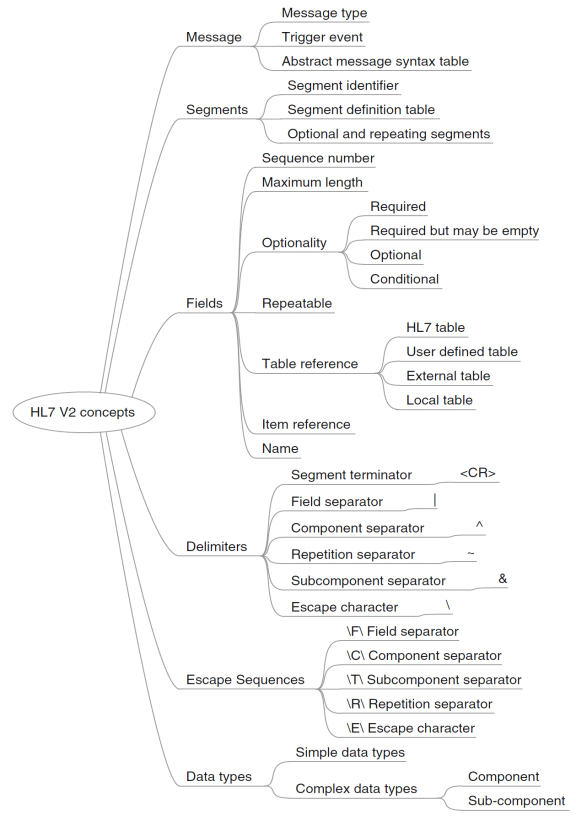
\includegraphics[width=1\textwidth]{HL7_V2_concepts.jpg}
	    \caption{Βασικές αρχές του προτύπου HL7 V2}
	    \label{fig:HL7_V2_concepts}
	\end{figure}
\newpage
	\begin{figure}[H]
	    \centering
	    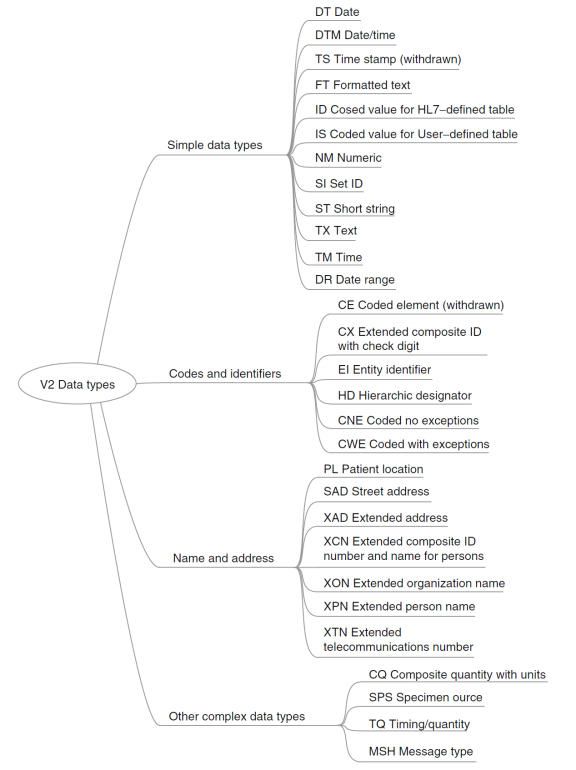
\includegraphics[width=1\textwidth]{HL7_V2_data_types.jpg}
	    \caption{Τύποι δεδομένων του προτύπου HL7 V2}
	    \label{fig:HL7_V2_data_types}
	\end{figure}
			
		\subsubsection{Το πρότυπο HL7, έκδοση 3}
		Σκοπός της έκδοσης 3 του προτύπου HL7 είναι η υποστήριξη των ροών εργασίας σε όλο το φάσμα της Υγειονομικής Περίθαλψης. Η ανάπτυξη της ξεκίνησε το έτος 1995 και διήρκεσε 10 χρόνια, δεδομένου ότι μπήκε στην `αγορά' εν έτη 2005. Υιοθέτησε μια διαφορετική προσέγγιση σε σχέση με τον προκάτοχο του, αφού βασίστηκε σε αντικειμενοστραφή λογική ενώ προσπάθησε παράλληλα και να περιορίσει την ευελιξία που υπήρχε στην έκδοση 2 με βασικό στόχο να εξαλείψει τα μειονεκτήματα τα οποία συνόδευαν την ευελιξία αυτή\cite{HL7V3ProductSuite}.
		
		Η πιο βασική διαφοροποίηση της εν λόγω έκδοσης αποτελεί το μοντέλο RIM (Reference Information Model), το οποίο πηγάζει από την αντικειμενοστραφή λογική που έχει υιοθετηθεί\cite{HL7RIM}. Το μοντέλο RIM περιγράφει τις κλάσεις που ανήκουν στο RIM και μπορούν να αναπαραστήσουν το σύνολο των μηνυμάτων HL7 V3, τις σχέσεις μεταξύ τους, το μοντέλο καταστάσεων και τα πεδία της εκάστοτε κλάσης. Παρέχει μια ρητή αναπαράσταση των σημασιολογικών και λεκτικών συνδέσμων μεταξύ της πληροφορίας στα πεδία των μηνυμάτων του HL7. Σύμφωνα με τον οργανισμό HL7 το μοντέλο αυτό προσφέρει υψηλή ακρίβεια και βοηθάει σημαντικά στην μείωση του κόστους υλοποίησης. Τα βασικότερα πεδία που συναντάμε στις κλάσεις του RMI φαίνονται στον πίνακα \ref{tab:HL7_V3_RMI_fields}.
	\begin{table}[h]
		\begin{center}
		    \begin{tabular}{|c|l|}
		    \hline
		    \rowcolor{grayy}
		    \textbf{Πεδίο} & \textbf{Λειτουργία}
		    \\ \hline
		     id & Ταυτοποίηση κάθε αντικειμένου (instance identifier)
		     \\ \hline
		     classCode & Εξειδίκευση της κλάσης βάσει ορισμών του HL7 V3
		     \\ \hline
		     code & Περιέχει το σχήμα κωδικοποίησης
		     \\ \hline
		     statusCode & Δείχνει την τρέχουσα κατάσταση του αντικειμένου
		     \\ \hline
		    \end{tabular}
		    \caption{Βασικά πεδία κλάσεων του μοντέλου RIM}
			\label{tab:HL7_V3_RMI_fields}
		\end{center}
	\end{table}
	
	Οι κύριες κλάσεις του μοντέλου RIM έχουν ως εξής\cite{gunther2006hl7}:
	\begin{itemize}
		\item \textbf{Act: } Κάθε μία πράξη ή ενέργεια που πραγματοποιείται είναι ένα Act (δηλαδή ανήκει στην κλάση act). Αποτελεί μια κλάση που περιλαμβάνει ένα τεράστιο εύρος ενεργειών, μερικά παραδείγματα είναι τα παρακάτω:
		\begin{itemize}
			\item Παρατηρήσεις π.χ. ιατρικές διαγνώσεις, ευρήματα εξετάσεων
			\item Γεγονότα π.χ. ραντεβού ασθενούς, εισαγωγή ασθενούς 
		\end{itemize}
		\item \textbf{ActRelationship: } Τα Acts συνδέονται μέσω της κλάσης ActRelationship.
		\item \textbf{Participation: } Ορίζει το περιβάλλον κάποιου Act (συγγραφέας, θέμα, τοποθεσία κτλπ.)
		\item \textbf{Entity: } Αποτελεί αναπαράσταση των φυσικών και μη οντοτήτων. Παραδείγματα οντοτήτων αποτελεί έναν ασθενής, ένας οργανισμός ή ακόμα και κάποιο νοσοκομείο.
		\item \textbf{Role: } Χρησιμοποιείται για να περιγράψει τους ρόλους που έχουν οι οντότητες σε κάποιο Act.
		\item \textbf{RoleLink: } Δείχνει τη σχέση που έχουν οι διάφοροι ρόλοι (Roles) μεταξύ τους.
	\end{itemize}
	Για να γίνουν πιο εύκολα κατανοητές οι παραπάνω κλάσεις καθώς και ο τρόπος με τον οποίο διασυνδέονται στο σχήμα \ref{fig:RMI_class_model} βλέπουμε το διάγραμμα κλάσεων\cite{gunther2006hl7}.
	\begin{figure}[h]
	    \centering
	    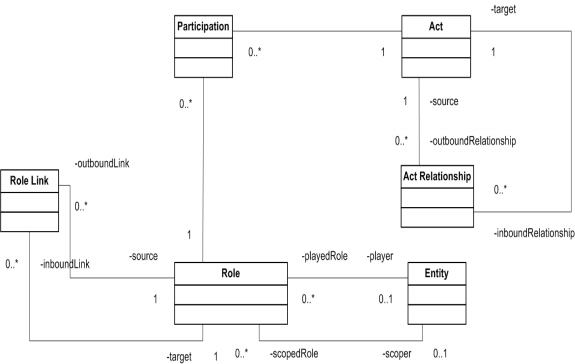
\includegraphics[width=1\textwidth]{RMI_class_model.jpg}
	    \caption{Διάγραμμα κλάσεων του μοντέλου RMI}
	    \label{fig:RMI_class_model}
	\end{figure}		
		
	Για λόγους πληρότητας στο σχήμα \ref{fig:HL7_V3_data_types} βλέπουμε τους διάφορους τύπους δεδομένων που υποστηρίζονται από το πρωτόκολλο HL7 V3 (στο σχήμα \ref{fig:HL7_V2_data_types} μπορείτε να δείτε τους τύπους για την έκδοση 2)
\newpage
	\begin{figure}[H]
	    \centering
	    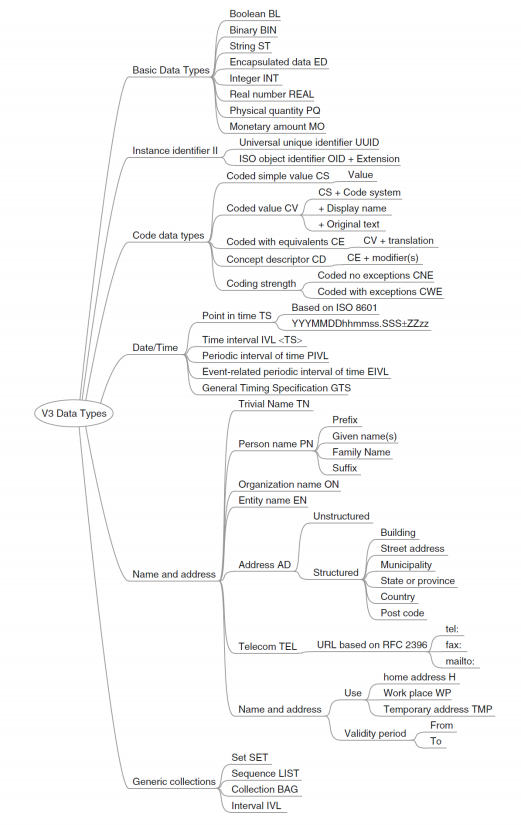
\includegraphics[width=1\textwidth]{HL7_V3_data_types.jpg}
	    \caption{Τύποι δεδομένων του προτύπου HL7 V3}
	    \label{fig:HL7_V3_data_types}
	\end{figure}
\newpage		
	\subsection{CDA Documents}
	

		
\section{Δυνατότητες διασύνδεσης με άλλα υποσυστήματα}

	\subsection{Ηλεκτρονική Συνταγογράφηση}
	
		Η διαδικασία της συνταγογράφησης φαρμάκων μπορεί να είναι ιδιαίτερα περίπλοκη και επιρρεπής σε λάθη, με
δυσμενείς επιπτώσεις για την ασφάλεια των ασθενών. Η πρόληψη των επιπλοκών που μπορούν να προκύψουν λόγω ακατάλληλης συνταγογράφησης είναι μία πρόκληση που αντιμετωπίζει το σύστημα υγείας σε παγκόσμιο επίπεδο. Οι λανθασμένες φαρμακευτικές αγωγές, οι παρενέργειες των φαρμάκων και η αποτυχία σωστής συνταγογράφησης που να συντελέσει στην θεραπεία του ασθενούς εκτός του γεγονότος ότι αποτελεί απειλή για την ασφάλεια του, οδηγεί σε σημαντικές δαπάνες για τα συστήματα υγειονομική περίθαλψης. Οι πληροφορίες σχετικά με το ιστορικό του ασθενούς, τις αλλεργίες, τις παρελθοντικές και τις τρέχουσες φαρμακευτικές αγωγές καθώς και τα εργαστηριακά αποτελέσματα του είναι άκρως απαραίτητα ώστε οι κλινικοί ιατροί να συνταγογραφήσουν την κατάλληλη φαρμακευτική αγωγή, αλλά είναι συχνά δεν είναι διαθέσιμα. \cite{prescribingErrors} Στην Ελλάδα ειδικότερα, υφίσταται το πρόβλημα της αλόγιστης ή πλασματικής συνταγογράφησης με αποτέλεσμα να  χρειάζονται μέτρα για την επαναφορά της αξιοπιστίας της διαδικασίας.  Χαρακτηριστικό παράδειγμα είναι τα στοιχεία του Υπουργείου Υγείας και Κοινωνικής Ασφάλισης, με βάση τα οποία το έτος 2009 εκτελεστήκαν στην Ελλάδα περίπου 100 εκατομμύρια ετησίως ενώ αντίστοιχα στην Δανία εκτελέστηκαν μόνο 15 εκατομμύρια συνταγές.


		Με τον όρο ηλεκτρονική συνταγογράφηση (e-prescription) σύμφωνα με το Εθνικό Σύστημα Υγείας στην Αγγλία αναφερόμαστε στην αξιοποίηση των ηλεκτρονικών συστημάτων για την διευκόλυνση και την ενίσχυσης της επικοινωνίας μίας ιατρικής εντολής ή συνταγής, βοηθώντας στην επιλογή, τη διαχείριση και την προμήθεια ενός φαρμάκου μέσω της γνώσης και υποστήριξης αποφάσεων, παρέχοντας μια διαδρομή ελέγχου για το σύνολο της διαδικασίας χρήσης των φαρμάκων.  Τα συστήματα ηλεκτρονικής συνταγογράφησης που προσφέρουν ηλεκτρονική υποστήριξη στους κλινικούς ιατρούς έχουν σχεδιαστεί για να βοηθήσουν στην περίπλοκη διαδικασία της συνταγογράφησης. \cite{Kierkegaard2013} Επιτρέπουν σε έναν γιατρό, έναν φαρμακοποιό, μία νοσηλεύτρια να διαβιβάσει χωρίς σφάλματα, ακριβείς και κατανοητές συνταγές ηλεκτρονικά, μέσα από τον φορέα παροχής υπηρεσιών υγείας, στο φαρμακείο.  \cite{eprescr}
		
		
		Τα συστήματα ηλεκτρονικής συνταγογράφησης μπορεί να έχουν λειτουργικές δυνατότητες για την παροχή βασικής υποστήριξης αποφάσεων, όπως ο έλεγχος για τυχόν αλλεργίες στα φάρμακα, βασικές κατευθυντήριες γραμμές για τη δοσολογία, τεστ για πιθανές αντιδράσεις μεταξύ φαρμάκων κ.λ.π. Τα συστήματα αυτά είναι ιδιαίτερα χρήσιμα στο τεχνικό κομμάτι της συνταγογράφησης κατάλληλων φαρμάκων, καθώς προσφέρουν λειτουργίες όπως ο υπολογισμός της σωστής δόσης ή ο εντοπισμός αλληλεπιδράσεων μεταξύ των φαρμάκων. \cite{Kart2008}

		Τα συστήματα ηλεκτρονικής συνταγογράφησης χωρίζονται σε δύο κατηγορίες:
		
		\begin{itemize}
		
		\item Τα αυτόνομα συστήματα (stand alone systems). Πρόκειται για λειτουργικά συστήματα τα οποία είναι εγκατεστημένα στους ηλεκτρονικούς υπολογιστές  και χρησιμοποιούνται είτε αυτόνομα είτε μέσω σύνδεσης στο διαδίκτυο.  Τα συστήματα αυτά χρησιμοποιούνται κυρίως για τον έλεγχο θεμάτων ασφάλειας και γίνεται προσπάθεια αντικατάστασης τους από τα ολοκληρωμένα συστήματα συνταγογράφησης.

		\item Τα ολοκληρωμένα συστήματα συνταγογράφησης (Electronic Health Record, EHR Systems). Στα συστήματα αυτά ο ιατρός έχει στην διάθεση του όλο το ιστορικό του ασθενούς, τα αποτελέσματα των εξετάσεων του και τα χρησιμοποιεί για να βοηθηθεί στην επιλογή της κατάλληλης δραστικής ουσίας. Οι συναγερμοί ασφαλείας στην περίπτωση αυτή είναι πιο εξειδικευμένοι και ακριβείς.  

		\end{itemize}
		

		Συνοπτικά τα συστατικά της ηλεκτρονικής συνταγογράφησης μπορούν να κατηγοριοποιηθούν σε βασικές δυνατότητες συνταγογράφησης, πληροφορίες για το πλάνο υγείας και τις κλινικές ειδοποιήσεις (clinical alerts).  Οι δυνατότητες συνταγογράφησης περιλαμβάνουν μια λίστα φαρμάκων, οδηγίες για τους ασθενείς, τον αριθμός των εγκεκριμένων ποσοτήτων, σχόλια του γιατρού που συνταγογραφεί προς τον φαρμακοποιό, καθώς και το πεδίο PRN. Οι πληροφορίες για το πλάνο υγείας του ασθενούς περιλαμβάνουν την ιατρική ασφάλεια που έχει και το ιστορικό των φαρμακευτικών αγωγών. Τέλος, οι κλινικές ειδοποιήσεις  βασίζονται στα δημογραφικά στοιχεία και στα στοιχεία του ιατρικού ιστορικού του ασθενούς και περιλαμβάνουν τις αντιδράσεις μεταξύ των φαρμάκων, τις αλλεργίες, τις προειδοποιήσεις για συγκεκριμένες ηλικιακές ομάδες και την κατάλληλη προσαρμογή της δόσης με βάση το βάρος του ασθενούς. \cite{prescribing} 
		
		
		Τα βασικά συστατικά ενός συστήματος ηλεκτρονικής συνταγογράφησης είναι \cite{Grossman2012}:

		\begin{itemize}

		\item Ο παραπέμπων ιατρός. Ο θεράπων ιατρός είναι ο κύριος χρήστης  του συστήματος. Για την σύνδεση του στο σύστημα ακολουθείται μιας διαδικασία επαλήθευσης ώστε να επιβεβαιωθεί η ταυτότητά του. 
Οι αναζητήσεις του θεράποντα ιατρού στην βάσης δεδομένων που περιέχει τους φακέλους των ασθενών πραγματοποιείται με τη χρήση ειδικών πληροφοριών για τον ασθενή, συνήθως το ΑΜΚΑ για Ελλάδα ή τον αριθμό κοινωνικής ασφάλισης (social security number) στον εξωτερικό. Μόλις προσπελαστεί το σωστό αρχείο του ασθενούς, ο ιατρός εξετάζει τις ιατρικές πληροφορίες που περιέχει και προσθέτει ή ενημερώνει μία συνταγή στον ιατρικό φάκελο.
		
		\item Ο κόμβος συναλλαγών. Αποτελεί τον κοινό σύνδεσμο μεταξύ όλων των φορέων (παραπέμπων ιατρός και φαρμακείο). Αποθηκεύει και διατηρεί ένα κύριο κατάλογο των ασθενών για να υπάρχει η δυνατότητα γρήγορης πρόσβασης στις ιατρικές πληροφορίες των ασθενών, καθώς και στην λίστα των φαρμακείων. Όταν ο παραπέμπων ιατρός ανεβάσει κάποια νέα συνταγή στον φάκελο του ασθενούς, τότε αυτή μεταφέρεται αυτόματα και στον κόμβο συναλλαγών. Ο κόμβος συναλλαγών θα στείλει αυτόματα τις πληροφορίες  με στο κεντρικό σύστημα διαχείρισης το οποίο θα απαντήσει με πληροφορίες σχετικά με την καταλληλότητα του ασθενή και το ιστορικό των φαρμακευτικών αγωγών του.  Ο κόμβος συναλλαγών έπειτα στέλνει τις πληροφορίες στον ιατρό έτσι ώστε να έχει τις απαραίτητες πληροφορίες που του χρειάζονται και να ολοκληρώσει και να εγκρίνει την συνταγή. 
		
		\item Το κεντρικό σύστημα διαχείρισης δεδομένων, στο οποίο βρίσκονται όλα τα στοιχεία ιατρικού φακέλου που ελέγχει την καταλληλότητα του ασθενή καθώς και της συνταγής. Το κεντρικό σύστημα διαχείρισης δεδομένων επικοινώνει με τον ιατρό και το φαρμακείο.
		
		\item Το φαρμακείο που έχει εγκατεστημένο το λογισμικό της ηλεκτρονικής συνταγογράφησης. Το φαρμακείο ανακτά την συνταγή από  το κεντρικό σύστημα διαχείρισης συναλλαγών μέσω του κόμβου συναλλαγών και έχει επιπλέον την ικανότητα να επικοινωνήσει με τον ιατρό και να τον ενημερώσει ότι η παραγγελία εκτελέστηκε. 
		
		\end{itemize}
		
		
		
		\subsubsection{Ηλεκτρονική Συνταγογράφηση στην Ελλάδα}
		
		Η ηλεκτρονική συνταγογράφηση στην Ελλάδα βασίζεται στις οδηγίες του νόμου 3892/2010 (ΦΕΚ 189 Α) «Ηλεκτρονική καταχώριση και εκτέλεση ιατρικών συνταγών και παραπεμπτικών ιατρικών εξετάσεων». Σε αυτόν το νόμο καταγράφονται τα ζητήματα ηλεκτρονικής συνταγογράφησης και τα ζητήματα των ηλεκτρονικών παραπεμπτικών.
		
		Ο υπεύθυνος φορέας στην Ελλάδα είναι η Γενική Γραμματεία Κοινωνικών Ασφαλίσεων του Υπουργείου Εργασίας, Κοινωνικής Ασφάλισης και Πρόνοιας. Το σύστημα υποστηρίζεται ηλεκτρονικά από την Ηλεκτρονική Διακυβέρνηση Κοινωνικής Ασφάλισης (ΗΔΙΚΑ Α.Ε.). Η ΗΔΙΚΑ αποτελεί μια ανώνυμη, μη κερδοσκοπικού χαρακτήρα του δημοσίου την οποία αποζημιώνουν οι εξυπηρετούμενοι φορείς για τις υπηρεσίες του παρέχει, όπως για παράδειγμα το έργο μισθοδοσίας των φορέων.  \cite{idika}
		
		Με τον όρο ηλεκτρονική συνταγογράφηση αναφερόμαστε στη παραγωγή, στην διακίνηση και στον έλεγχο των ιατρικών συνταγών και των παραπεμπτικών για ιατρικές πράξεις, με τη χρήση τεχνολογίας ηλεκτρονικών υπολογιστών και επικοινωνιών, έτσι ώστε να διασφαλίζεται η ασφάλεια, η εγκυρότητα και η διαφάνεια στις πληροφορίες που διακινούνται. Ουσιαστικά, το σύστημα περιλαμβάνει ένα αριθμό από διαδικασίες που σχετίζονται με τη δημιουργία, την εκτέλεση, τη διαχείριση, τον έλεγχο, την εκκαθάριση και την εξόφληση μιας φαρμακευτικής συνταγής ή ενός παραπεμπτικού για ιατρικές πράξεις. Διέπει όλα τα συστήματα και τις τοποθεσίες που εμπλέκονται όπως τα τακτικά ιατρεία των νοσοκομείων ή τα ιδιωτικά ιατρεία, τα κέντρα υγείας, τις κλινικές, τα διαγνωστικά κέντρα, τα φαρμακεία και τα ασφαλιστικά ταμεία.


		
		Το ολοκληρωμένο σύστημα ηλεκτρονικής συνταγογράφησης στην Ελλάδα εξυπηρετεί τους εξής σκοπούς:
		
		\begin{itemize}

		\item  Βοηθά στον αποτελεσματικό εκσυγχρονισμό του συστήματος της φαρμακευτικής περίθαλψης. Οι χειρόγραφες συνταγές έχουν αντικατασταθεί από τις ηλεκτρονικές και η διαδικασία έχει αυτοματοποιηθεί.
		 
		\item Συντελεί στην ταυτοποίηση και τον έλεγχο των εμπλεκομένων για να διασφαλίσει την ακεραιότητα της διαδικασίας και την ευρεία και επιτυχημένη επιχειρησιακή λειτουργία της ηλεκτρονικής συνταγογράφησης.
		
		\item Βελτιώνει την ασφάλεια και την ποιότητα της φροντίδας του ασθενούς. Με την αύξηση του όγκου των φαρμάκων και της πολυπλοκότητα των ιατρικών αναγκών των ασθενών, εφίσταται αυξημένος κίνδυνος σφαλμάτων και παρενεργειών. Η ηλεκτρονική συνταγογράφηση μπορεί να βελτιώσει την ασφάλεια και την ποιότητα της φροντίδας του ασθενούς και να μειώσει τον αριθμό των λαθών
		
		\item Εισάγει και αξιοποιεί τις λειτουργίες της ηλεκτρονικής συνταγογράφησης στην καθημερινή πρακτική.

		\end{itemize}

	\subsubsection{E-prescription }
	
		Το ελληνικό σύστημα ηλεκτρονικής συνταγογράφησης,  το επονομαζόμενο e-precription, καθιερώθηκε το 2013. Πλέον καλύπτει περισσότερο  από το 95\% του συνόλου των συνταγών που γράφονται . Το e-precription δημιουργήθηκε με σκοπό να παρέχει τις εξής λειτουργίες: την ηλεκτρονική καταχώρηση και διαχείριση των συνταγών, την ενίσχυση της γνώσης μέσω της δυνατότητας άμεσης πρόσβασης στις πληροφορίες των φαρμάκων, την υποστήριξη λήψης αποφάσεων καθώς βοηθά την επιλογή των φαρμάκων με διάφορες ειδοποιήσεις, την υποστήριξη κατά την διοίκηση, την δημιουργία ηλεκτρονικών συνδέσμων μεταξύ των νοσοκομείων και των φαρμακείων, τις βελτιώσεις στις ήδη υπάρχουσες εργασιακές διαδικασίες, και τέλος την ανάπτυξης μιας διαδρομή ελέγχου για το σύνολο της χρήσης των φαρμάκων.  \cite{miller}
		
		Το e-prescription πραγματοποιεί την ηλεκτρονική επεξεργασία των συνταγών για όλους τους ασθενείς, οι οποίοι είναι ασφαλισμένοι σε κάποιον από τους εθνικούς φορείς ασφαλίσεων.Το σύστημα εστιάζει ιδιαιτέρως στην βελτίωση της ασφάλειας των ασθενών, την καλύτερη αξιοποίηση των πόρων και στην διαλειτουργικότητα με άλλα εθνικά ή ευρωπαϊκά συστήματα. Είναι διαθέσιμο μέσω του διαδικτύου (internet) και αποτελεί ένα αυτόνομο ηλεκτρονικό σύστημα εισόδου στο οποίο κάθε υποβολή συνταγής είναι ασφαλής και αναγνωρίζεται από έναν μοναδικό αριθμό. Στο σχήμα \ref{fig:prescr} απεικονίζεται η συνολική δομή του συστήματος. \cite{pangalos}
		
		Ο θεράπων ιατρός δημιουργεί τις συνταγές οι οποίες αποθηκεύονται στην εθνική βάση του συστήματος e-prescription , η οποία βρίσκεται στην ΗΔΙΚΑ. \cite{idika}Όταν ένα φαρμακείο θέλει να εκτελέσει μία συνταγή την  "διαβάζει" από την κεντρική βάση. Οι πληροφορίες ου βρίσκονται στην βάση δεδομένων είναι διαθέσιμες (μέσω ασφαλούς on-line πρόσβασης, ή εξειδικευμένων περιοδικών αναφορών) σε όλα τα σχετικά και ενδιαφερόμενα μέρη (Οργανισμοί Ασφάλισης Υγείας, Υπουργείο Υγείας, εποπτικές αρχές, κλπ). Οι συνταγές που έχουν εκτελεστεί από τα φαρμακεία  ελέγχονται από τους οργανισμούς ασφάλισης, ενώ το σύστημα e-prescription χρησιμοποιείται για να διασταυρώνονται οι έλεγχοι. \cite{papala}

	Η εφαρμογή του e-prescription είναι μία διαδικτυακή εφαρμογή. Στο σύστημα έχουν πρόσβαση μόνο εξουσιοδοτημένοι χρήστες (ιατροί, φαρμακοποιοί, κλπ), οι οποίοι αναγνωρίζονται και αποκτούν άδεια πρόσβασης μετα την χρήση κατάλληλων διαπιστευτηρίων. για χωροθέτηση και αδειοδότηση.
	
	Ο θεράπων ιατρός δημιουργεί συνταγές, οι οποίες παρέχουν όλες τις απαραίτητες πληροφορίες τόσο για τους ιατρικούς όσο και για τους διοικητικούς σκοπούς.  Στις πληροφορίες αυτές συμπεριλαμβάνεται ο αριθμός κοινωνικής ασφάλισης  του ασθενούς και του ιατρού , ο κωδικός της διάγνωσης (που κωδικοποιείται στο ICD-10), τα στοιχεία του καθορισμένου φαρμάκου (ποσότητα, δοσολογία, κ.λ.π.), το ποσοστό συμμετοχής του ασθενή στην πληρωμή του φαρμάκου και άλλα στοιχεία.  Αυτές οι πληροφορίες εκτός από την βοήθεια που προσφέρουν στους ιατρούς, συντελούν στην γνώση των λεπτομερειών της διαδικασίας συνταγογράφησης εύκολα και σε πραγματικό χρόνο. Η δυνατότητα αυτή καθιστά το e-prescription σύστημα ένα ισχυρό εργαλείο όχι μόνο για την ενίσχυση της παρακολούθησης της δημόσιας υγείας και τον σχεδιασμό της, αλλά και για την βελτίωση του διοικητικού έλεγχου
και τη διαφάνεια των δαπανών των φαρμάκων. Τέλος, το σύστημα e-prescription παρέχει στους ασθενείς την δυνατότητα να  επιλέξουν, το φάρμακο που επιθυμούν ή μπορούν να αντεπεξέλθουν οικονομικά από μια λίστα ισοδυνάμων φαρμάκων στην οποία, συμπεριλαμβάνονται και τα γενόσημα φάρμακα. 

	\begin{figure}[h]
	    \centering
	    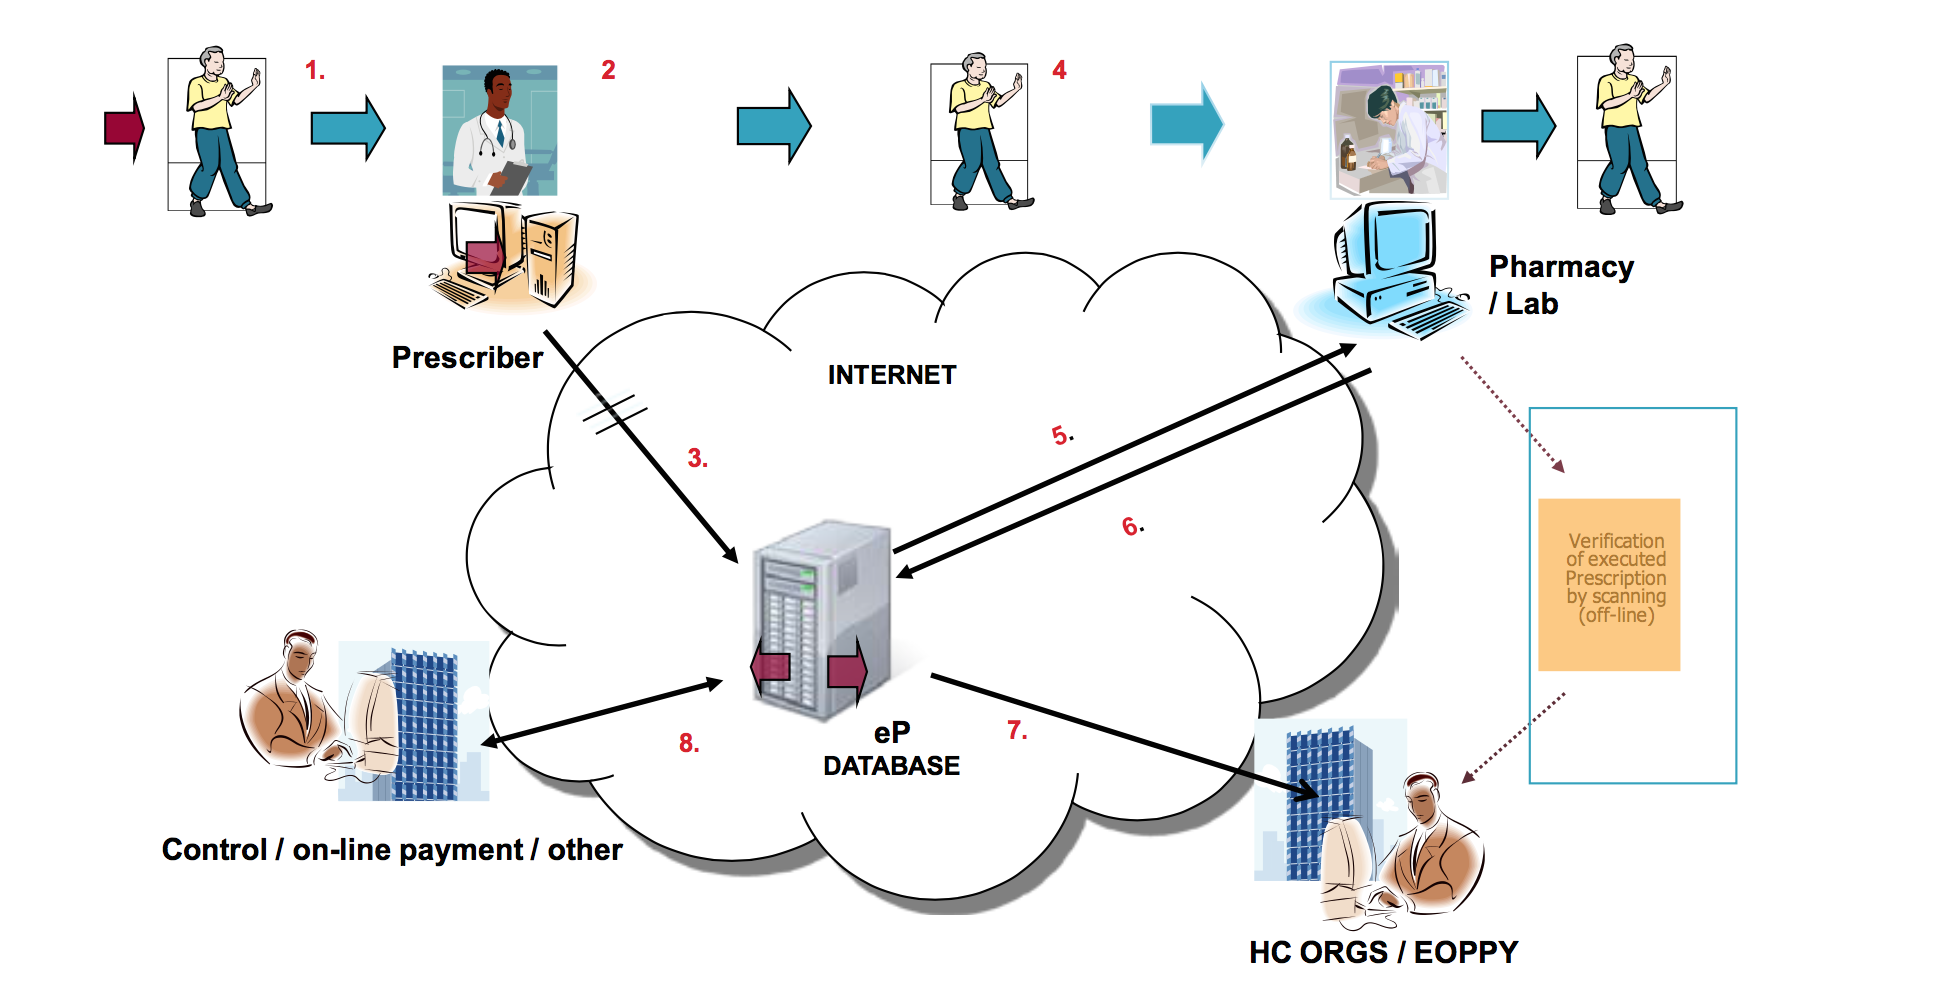
\includegraphics[width=0.7\textwidth]{e-prescr.png}
	    \caption{Το σύστημα E-prescription στην Ελλάδα. }
	    \label{fig:prescr}
	\end{figure}


	

	
	\subsection{Ηλεκτρονικός Ιατρικός Φάκελος (EMR)}
	

		Στην σύστημα υγείας η πληρότητα και η διαθεσιμότητα των δεδομένων και της πληροφορίας είναι ζωτικής σημασίας. Ημιτελείς πληροφορίες μπορούν να έχουν ως αποτέλεσμα κακή διάγνωση και θεραπεία, σπατάλη χρημάτων και πόρων ακόμα και να επιφέρουν καταστάσεις οι οποίες να απειλούν τη ζωή. Ο όγκος των πληροφοριών που σχετίζονται με την φροντίδα του ασθενούς έχει πολλαπλασιαστεί τα τελευταία χρόνια, γεγονός που οφείλεται σε μεγάλο ποσοστό στην ενσωμάτωση αυξημένου αριθμού εργαστηριακών και παρακλινικών εξετάσεων στους φακέλους των ασθενών.
	
		Ο ηλεκτρονικός ιατρικός φακέλου είναι ένα σύστημα σχεδιασμένο ώστε να υποστηρίζει την απόλυτη διαθεσιμότητα και την ακρίβεια ιατρικών ή άλλων πληροφοριών με σκοπό την παροχή ιατρικής περίθαλψης. Ο ηλεκτρονικός ιατρικός φάκελος ασθενούς είναι μία διαρκώς εξελισσόμενη έννοια και καθορίζεται ως μια συλλογή από ιατρικές πληροφορίες ιδιωτών ή πληθυσμών. Είναι αποθηκευμένος σε ψηφιακή μορφή, έχει την ικανότητα να διαμοιράζεται μεταξύ διαφορετικών ιατρικών λογισμικών και μπορεί να μεταφερθεί μέσω του δικτύου. Ένας ηλεκτρονικός φάκελος μπορεί να περιλαμβάνει μεγάλο πλήθος δεδομένων σε πλήρη ή περιληπτική μορφή, όπως δημογραφικά στοιχεία, ιατρικό ιστορικό φαρμακευτική αγωγή και αλλεργίες, προσωπικά στοιχεία όπως βάρος, ύψος, φύλο και άλλα.
		
		Σε αυτό το σημείο θα πρέπει να κάνουμε τον διαχωρισμό του ηλεκτρονικού ιατρικού φακέλου(EMR) και του ηλεκτρονικού φακέλου υγείας(EHR). O ηλεκτρονικός φάκελος υγείας (EHR) είναι μια εξελισσόμενη έννοια 
που αποθηκεύει ψηφιακά ένα υποσύνολο δεδομένων ή όλα τα δεδομένα σχετικά με τις ιατρικές πράξεις που έγιναν κατά τη διάρκεια της ζωής ενός ατόμου με σκοπό την υποστήριξη της ποιοτικής, προσβάσιμης και αποτελεσματικής συνέχειας στην παροχή υπηρεσιών υγείας. Ο ηλεκτρονικός ιατρικός φάκελος σε αντίθεση ορίζεται ως το αρχείο του ασθενούς που δημιουργήθηκε από τους παρόχους για συγκεκριμένες επισκέψεις του ασθενή σε νοσοκομεία και περιπατητική περιβάλλοντα, και η οποία μπορεί να χρησιμεύσει ως πηγή δεδομένων για τον ηλεκτρονικό φάκελο υγείας (EHR). Ο ηλεκτρονικός φάκελος υγείας (EHR) δημιουργείται και διατηρείται εντός ενός θεσμικού οργάνου, όπως ένα νοσοκομείο, ένα ολοκληρωμένο δίκτυο διανομής,μία κλινική, ή ένα γραφείο ιατρού για να δώσει σε όλους τους εμπλεκόμενους στην ιατρική φροντίδα πρόσβαση ιατρικό ιστορικό του ασθενούς.
	
	
		Ο κλασσικός ηλεκτρονικός ιατρικός φάκελος πρέπει κάθε χρονική στιγμή να περιέχει τουλάχιστον την επίσκεψη-επαφή του ασθενούς, το ιατρικό ιστορικό, τη διάγνωση, τη νοσηλεία (συνταγογράφηση, αποτελέσματα εργαστηριακών εξετάσεων ), τα δημογραφικά στοιχεία του ασθενούς (Όνομα, ΑΜΚΑ, Ασφαλιστικός φορέας, ομάδα αίματος κ.τ.λ.).


Το λογισμικό του ηλεκτρονικού φακέλου υγείας ουσιαστικά είναι ένα σύστημα διαχείρισης ιατρικών φακέλων που βασίζεται σε ηλεκτρονικούς υπολογιστές. Το γεγονός αυτό έχει ως αποτέλεσμα να αποθηκεύονται και να ανακτώνται δεδομένα γρήγορα και με ασφάλεια. Επιπλέον, τα δεδομένα επεξεργάζονται εύκολα και γρήγορα και μπορούν να μεταφερθούν σε οποιαδήποτε σύστημα, σε οποιαδήποτε απόσταση. Το σύστημα καταγραφής των δεδομένων γίνεται πιο αποτελεσματικό και περισσότερο πλήρες. Ο ηλεκτρονικός ιατρικός φάκελος εμπεριέχει μία πληθώρα δεδομένων, τα οποία έχουν διαφορετική μορφή. Το ιστορικό, η κλινική εξέταση και τα αποτελέσματα εργαστηριακών εξετάσεων, είναι σε μορφή κειμένου, οι εξετάσεις του ασθενούς (ακτινογραφίες, τομογραφίες - αξονικές, μαγνητικές, απλές - υπέρηχοι κ.α.) είναι σε μορφή στατικών εικόνων, τα ηλεκτροκαρδιογραφήματα είναι σε μορφή βιοσημάτων ,τα αποτελέσματα των ενδοσκοπικών εξετάσεων (γαστροσκόπηση κ.α. ) είναι σε μορφή βίντεο κ.λ.π.  Στον ηλεκτρονικό ιατρικό φάκελο , όλα τα δεδομένα ενσωματώνονται στον φάκελο του ασθενούς χωρίς να παίζει σημαντικό ρόλο η μορφή τους. Σε διάφορα σημεία του κειμένου του ιστορικού και της κλινικής εξετάσεως ενσωματώνονται ακτινολογικές ή βιοχημικές εξετάσεις, πράγμα που κάνει αμέσως εμφανή την συσχέτιση των εν λόγω εξετάσεων με την γενικότερη κατάσταση του ασθενούς.

Μερικά από τα πιο ουσιαστικά πλεονεκτήματα της χρήσης ενός συστήματος ηλεκτρονικού ιατρικού φακέλου είναι τα εξής
\begin{itemize}

\item Κέρδος χρόνου κατά την αναζήτηση και την συμπλήρωση στοιχείων του ιατρικού φακέλου. Η διείσδυση των τεχνολογιών αιχμής στον ιατρικό κόσμο εκσυγχρονίζεις την διαδικασία και κρατώντας όλα τα στοιχεία συγκεντρωμένα και με δυνατότητα άμεσης πρόσβασης - αναζήτησης επιταχύνουμε πολύ τις διαδικασίες.


\item

\item


\end{itemize}



Η ασφάλεια των ιατρικών δεδομένων είναι ένα σημαντικότατο θέμα για το οποίο, η
τεχνολογία μέσω του ηλεκτρονικού ιατρικού φακέλου έχει δώσει ουσιαστικές λύσεις, οι οποίες
μάλιστα μπορεί να θεωρηθούν αποτελεσματικότερες από αυτές που μέχρι σήμερα εφαρμόζονται
για την τήρηση και φύλαξη των ιατρικών φακέλων των ασθενών.
Στον ηλεκτρονικό ιατρικό φάκελο δίνεται ιδιαίτερη έμφαση στην προστασία των
προσωπικών δεδομένων τα οποία αρχειοθετούνται. Φυσικά λόγω της ευαισθησίας των
προσωπικών στοιχείων, πληρούνται όλες εκείνες οι προϋποθέσεις ασφαλείας που εξασφαλίζουν
το αδιάβλητο των δεδομένων. 


	
	
	\subsection{epSOS}
	
		Η ανάγκη διασύνδεσης των συστημάτων υγείας και των πολιτικών που ακολουθούνται σε κάθε κράτος σχετικά με την υγεία στην Ευρωπαϊκή Ένωση, γίνεται όλο και πιο πιεστική, λόγω της αυξημένης κινητικότητας των ασθενών και των επαγγελματιών του ιατρικού τομέα και της διάδοσης των νέων ιατρικών τεχνολογιών και τεχνικών που αφορούν την τεχνολογία της πληροφορίας. Η διασύνδεση των διάφορων συστημάτων υγείας είναι απαραίτητη για την καλύτερη ποιότητα αλλά και την άμεση πρόσβαση των πολιτών στη διασυνοριακή περίθαλψη.  Πολλά κράτη μέλη της Ευρωπαϊκής Ένωσης έχουν αναπτύξει ηλεκτρονικά συστήματα σχετικά με τα αρχεία των ασθενών. Ο ηλεκτρονικός ιατρικός φάκελος του ασθενούς και η ηλεκτρονική συνταγογράφηση είναι δύο πολύ σημαντικά συστήματα τα οποία προάγουν την ασφαλή και αξιόπιστη ιατροφαρμακευτική περίθαλψη.	 	
	 	
	 	Η Ευρωπαϊκή Ένωση στα πλαίσια του στόχου της επικοινωνίας και της συνεργασίας των χωρών που εντάσσονται σε αυτή και την ύπαρξη κοινών οδηγιών στον τομέα της υγείας, τον Ιούλιο του 2008 σε συνεργασία με τους δημόσιους φορείς που έχουν αρμοδιότητα τις ηλεκτρονικές υπηρεσίες υγείας (ηλεκτρονικός ιατρικός φάκελος, ηλεκτρονικής συνταγογράφησης) ξεκίνησε ένα σημαντικό έργο, τον ευρωπαϊκό πιλότο epSOS (Έξυπνες Ανοιχτές Ηλεκτρονικές Υπηρεσίες για τους Ευρωπαίους Ασθενείς). Ο κύριος στόχος του epSOS είναι η ανάπτυξη ενός πρακτικού πλαισίου ηλεκτρονικής υγείας και κατάλληλων  υποδομών  στον τομέα της  Πληροφορικής και των Επικοινωνιών που θα επιτρέπουν την ασφαλή πρόσβαση των διάφορων μη εθνικών ευρωπαϊκών συστημάτων υγειονομικής περίθαλψης στις πληροφορίες αναφορικά με την υγεία του ασθενούς. Το epSOS είναι ένα έργο για την προώθηση της δια-λειτουργικότητας της ηλεκτρονικής υγείας , το οποίο χρηματοδοτεί η Ευρωπαϊκή Ένωση και θέλει να χτίσει μια υποδομή υπηρεσιών, που θα επιτρέπει  τη διασυνοριακή διαλειτουργικότητα των συστημάτων ηλεκτρονικών μητρώων υγείας στην Ευρώπη, χωρίς να καταπατά όμως νομοθετικές ρυθμίσεις ή να υπερβαίνει τα ήδη υπάρχουσα εθνικά συστήματα. \cite{Dogac2012}


		Το epSOS αποτελείται από δύο χωριστές υπηρεσίες ηλεκτρονικής υγείας, τον ιατρικό φάκελο ασθενούς (patient medical record) και την ηλεκτρονική συνταγογράφηση (e-prescription),  για τις οποίες αναζητούνται δια-λειτουργικές μέθοδοι στη διασυνοριακή επικοινωνία. Ειδικότερα, ο ιατρικός φάκελος ασθενούς  (patient medical record) στα πλαίσια του epSOS αποτελείται από στοιχεία τα οποία εμπεριέχουν γενικές πληροφορίες για τον ασθενή (π.χ. όνομα, ηλικία, γένος), σημαντικά κλινικά δεδομένα (π.χ. αλλεργίες, χρόνιες ασθένειες, χειρουργικές επεμβάσεις) , καθώς και τα τρέχοντα αλλά και παλαιότερα φαρμακευτικά σκευάσματα που λάμβανε. Ο φάκελος ασθενούς παρέχει τις βασικές πληροφορίες, οι οποίες βοηθούν τους επαγγελματίες του τομέα της υγείας να λάβουν σωστότερες και πιο ασφαλείς αποφάσεις σχετικά με την θεραπεία και τα φάρμακα που θα ακολουθήσουν οι ασθενείς. Οι πληροφορίες αυτές πρέπει να παρέχονται στην γλώσσα των εκάστοτε γιατρών, ώστε να μην προκύπτουν γλωσσικά εμπόδια. Η ηλεκτρονική συνταγογράφηση αφορά τη συνταγογράφηση των φαρμάκων με χρήση κατάλληλου λογισμικού και την ηλεκτρονική διαβίβασή τους. Στην ηλεκτρονική συνταγογράφηση η διαλειτουργικότητα μεταξύ των εθνικών συστημάτων είναι απαραίτητη όταν έχουμε έναν ασθενή ο οποίος χρειάζεται κάποιο φάρμακο, το οποίο έχει ήδη συνταγογραφηθεί σε κάποια άλλη χώρα.  Ο φαρμακοποιός θα πρέπει να αποκτήσει ηλεκτρονική πρόσβαση στη συνταγή, και όταν το φάρμακο αγοραστεί, το ηλεκτρονικό σύστημα θα πρέπει να ενημερώσει σχετικά με τα διανεμημένα φάρμακα το σύστημα υγειονομικής περίθαλψης της χώρας του ασθενούς. \cite{epSOS}
		
		 Το epSOS επιτυγχάνει την ασφαλή πρόσβαση των ασθενών σε πληροφορίες σχετικά με την υγεία τους για τα διάφορα ευρωπαϊκά συστήματα υγείας. Το σύστημα είναι φτιαγμένο για να εξυπηρετήσει έναν πολίτη της Ευρωπαϊκής Ένωσης  που ενώ είναι κατοικεί σε μια συγκεκριμένη χώρας δέχεται τακτικά υπηρεσίες υγείας σε μια άλλη χώρα εξαιτίας του καθώς εργάζεται σε αυτή τη χώρα ή βρίσκεται προσωρινά σε μία άλλη χώρα (π.χ. για τουρισμό ) και είναι ανάγκη να εκτελέσει μία ιατρική συνταγή της χώρας του ή χρειάζεται επείγουσα ιατρική περίθαλψη. Το epSOS παρέχει την κοινοτική οδηγία για τη διασυνοριακή ιατρική περίθαλψη, η οποία θα πρέπει να ενσωματωθεί στο εθνικό δίκαιο των κρατών μελών τα επόμενα χρόνια και επιπροσθέτως προτείνει τεχνικές λύσεις σε όλα τα επίπεδα δια-λειτουργικότητας, όπως και σε θέματα πολιτικής και σε νομικά ζητήματα. επεκτείνεται πέρα από την έκδοση συστάσεων, μοντέλων οργάνωσης, και εργαλείων λογισμικού  στην  δοκιμή των αποτελέσματα αυτών μέσω πραγματικών πιλοτικών εφαρμογών σε πολλές ευρωπαϊκές περιφέρειες και χώρες.
		 


\section{Eligibility as a Service}

			\subsection{Motivation}
			
						
			Η πρωταρχική ευθύνη της υπηρεσίας μετάγγισης αίματος είναι να παρέχει ένα ασφαλές και επαρκές απόθεμα αίματος και προϊόντων που παράγονται από το αίμα. Θα πρέπει να διασφαλίζεται ότι τα προϊόντα που προέρχονται από δωρεές αίματος παρουσιάζουν ελάχιστο κίνδυνο ύπαρξης οποιασδήποτε μόλυνσης, που θα μπορούσε να μεταδοθεί μέσω μετάγγισης. Επίσης πρέπει να εξασφαλίζει ότι η υγεία του αιμοδότη δεν θα επιβαρυνθεί με οποιοδήποτε από τη δωρεά αίματος. Όλοι οι υποψήφιοι αιμοδότες αξιολογούνται για την καταλληλότητά τους να δωρίσουν αίμα, σε κάθε περίπτωση δωρεάς. 
		
		Οι βασικές φάσεις ελέγχου του αίματος είναι οι εξής:
		\begin{itemize}
		\item Φάση 1: Συμπλήρωση χειρόγραφου ερωτηματολογίου σχετικά με το ιστορικό υγείας του ασθενούς (βλ. παράρτημα \ref{Donor Questionnaire}).
		\item Φάση 2: Εξέταση του εθελοντή αιμοδότη από ιατρό και βασικές εξετάσεις (μέτρηση πίεσης, έλεγχος αιμοσφαιρίνης) και ερωτήσεις σχετικά με το ιατρικό ιστορικό του αιμοδότη.
		\item Φάση 3: Μετά την αιμοληψία, το αίμα περνάει μοριακούς και μικροβιολογικούς ελέγχους.
		\end{itemize}		 
		
		Οι πληροφορίες που παρέχονται από 164 χώρες για την παγκόσμια Βάση Δεδομένων για την ασφάλεια αίματος δείχνουν ότι πραγματοποιούνται περισσότερες από 92 εκατομμύρια αιμοδοσίες ετησίως\cite{WorldHealth}. Επιπλέον, τουλάχιστον 13 εκατομμύρια υποψήφιοι δότες απορρίπτονται πριν προλάβουν να φτάσουν στην αιμοληψία, δηλαδή στις φάσεις 1 και 2 όπως περιγράφηκαν παραπάνω\cite{safety}. Οι λόγοι απόρριψης κατά τις φάσεις αυτές, οι οποίοι και θα εξεταστούν στην παρούσα διπλωματική, έχουν να κάνουν με το ιατρικό ιστορικό του ασθενή (χρόνιες ασθένειες, αλλεργίες κ.λ.π.), με υπάρχουσες ιατρικές καταστάσεις (λοιμώξεις, λήψη αντιβίωσης, λήψη φαρμάκων που σε καθιστούν ακατάλληλο για  αιμοδοσία κ.λ.π.) και με καταστάσεις της προσωπικής ζωής του εθελοντή (π.χ. ομοφυλοφιλία). Το υπερβολικά μεγάλο ποσοστό απορρίψεων 14.13\% τονίζει την ανάγκη να μειωθεί ο αριθμός των περιπτώσεων της προσωρινής απόρριψης (με τον όρο προσωρινή απόρριψη, αναφερόμαστε σε προσωρινή αναβολή της αιμοδοσίας που συμβαίνει στις φάσεις 1, 2 λόγω προσωρινής ακαταλληλότητας των δοτών).

		Το ποσοστό αυτό, γίνεται ιδιαίτερος σημαντικό και ζημιογόνο οικονομικά αν κάνουμε μία ανάλυση των επιμέρους κοστών της αιμοδοσίας, δεδομένου του γενικότερου υψηλού κόστους κατά τη διαδικασίας της αιμοδοσίας. Στη συνέχεια θα παρουσιάσουμε την μέση τιμή αυτών των κοστών, όπως υπολογίσθηκε από το ελληνικό Υπουργείο Υγείας,το 2011\cite{Fragoulakis}. Στα κόστη περιλαμβάνεται το κόστος μηχανογράφησης (απογραφή και συντήρηση) των κέντρων αίματος, η τιμή των διαφόρων τύπων εξοπλισμού καθώς και το υπόλοιπο του κύκλου ζωής (που μετράται σε έτη) για τον ιατρικό εξοπλισμό. Επίσης, μετρώνται τα πάγια κόστη των μονάδων τα οποία σχετίζονται με την ηλεκτρική ενέργεια,  τον καθαρισμό, την ασφάλεια, την διαχείριση και όλες τις άλλες υποστηρικτικές υπηρεσίες που διατίθενται για τα κέντρα αίματος. Στον πίνακα \ref{tab:blood_collection_cost_greece} αναφέρονται αναλυτικά τα κόστη, των φάσεων 1 και 2 για την συλλογή 1 μονάδας αίματος στην Ελλάδα.
		
	\begin{table}[h]
		\centering
		\begin{tabular}{|l|c|}
		    \hline
		    \rowcolor{grayy}
		    \textbf{Περιγραφή} & \textbf{Μέσο κόστος}
		    \\ \hline
		     Προσωπικό & 46.86
		     \\ 
		     Γενικά έξοδα & 2.88
		     \\ 
		     Αναλώσιμα & 1.09
		     \\ 
		     Μηχανογράφηση & 0.92
		     \\
		     Σακούλα αίματος & 12.30
		     \\
		     Εξοπλισμός & 0.04
		     \\ 
		     Έμμεσο κόστος & 34.00
		     \\ \hline
		     Συνολικό κόστος & 98.07	
		     \\ \hline
		\end{tabular}
		\caption{Κόστος για την συλλογή 1 μονάδας αίματος στην Ελλάδα.}
		\label{tab:blood_collection_cost_greece}
	\end{table}
		
		Παρατηρούμε ότι το συνολικό κόστος για τις φάσεις 1 και 2 είναι 98.07 € ανά μονάδα αίματος.  Με βάση το ποσοστό απόρριψης 14.13\% βλέπουμε ότι για κάθε 100 αιμοδοσίες έχουμε 1,385.73 € έξοδα για περιπτώσεις στις οποίες δεν θα πραγματοποιηθεί ποτέ αιμοληψία. Σε αυτό το σημείο πρέπει να τονίσουμε, ότι δεν έχουν συμπεριληφθεί όλα τα κόστη στην μελέτη μας, παρά μόνο τα απολύτως διακριτά και ξεκάθαρα μετρήσιμα.
	
		Πέραν του οικονομικού μέρους, μια άλλη πολύ σημαντική παράμετρος είναι η άσκοπη κατανάλωση χρόνου τόσο του ιατρικού προσωπικού του αιμοδοτικού κέντρου, όσο και των εθελοντών αιμοδοτών. Οι εθελοντές αιμοδότες καταναλώνουν αρκετό χρόνο για τον προγραμματισμό, την μετάβαση στο αιμοδοτικό κέντρο, την αναμονή και για την διαδικασία αιμοδοσίας.  Δεδομένου ότι το μεγαλύτερο ποσοστό είναι εργαζόμενοι, ο χρόνος αυτός είναι σημαντικός και είναι επιθυμητό να αποφευχθεί η περιττή ταλαιπωρία που προκύπτει για τους δωρητές λόγω προσωρινής τους απόρριψης. Η αυτοματοποιημένη και πλήρως μηχανογραφημένη προσωρινή απόρριψη ενός εθελοντή αιμοδότη, θα εξασφαλίσει μείωση της σπατάλης του χρόνου αυτού.
		
		Μία επιπλέον πολύ σημαντική παράμετρος αποτελεί το ποσοστό επιστροφής των εθελοντών αιμοδοτών μετά από μία προσωρινή απόρριψη. Μελέτες έχουν δείξει ότι οι περισσότεροι εθελοντές δεν επιστρέφουν αν απορριφθούν μία φορά. Πιο συγκεκριμένα, μόλις το 11\% επιστρέφει μετά την απαιτούμενη περίοδο για να πραγματοποιήσει δωρεά αίματος\cite{halperin1998effect}.
	
		
	\subsection{Decision Support Systems \& Clinical Decision Support}
		Τα συστήματα υποστήριξης αποφάσεων (DSS - Decision Support Systems) μπορούν να οριστούν ως εφαρμογές λογισμικού οι οποίες παρέχουν υποστήριξη κατά την διαδικασία λήψης αποφάσεων, παρέχοντας βοήθεια στους χρήστες να κατανοήσουν τις επιπτώσεις των δράσεών τους\cite{french2000decision}. Τα DSS βρίσκουν χρήση σ' ένα ευρύ φάσμα εφαρμογών και εξυπηρετούν τη διαχείριση, τη λειτουργία αλλά και τα επίπεδα σχεδιασμού ενός συστήματος ή οργανισμού. Τα συστήματα υποστήριξης λήψης αποφάσεων μπορεί να είναι είτε πλήρως μηχανογραφημένα, είτε να διαχειρίζονται από ανθρώπινο δυναμικό  ή να αποτελούν συνδυασμό και των δύο (υβριδικά) \cite{miller}. 
		
		Τα συστήματα υποστήριξης λήψης κλινικών αποφάσεων (CDS) παρέχουν στους κλινικούς γιατρούς, στο προσωπικό, στους ασθενείς, και σε άλλα άτομα με γνώσεις σχετικές με αντικείμενα του τομέα υγείας, υποστήριξη στα κλινικά καθήκοντα τα οποία είναι συσχετισμένα με την διαδικασία απόφασης, με σκοπό  την ενίσχυση της υγείας και της υγειονομικής περίθαλψης\cite{clinicalDecision}. Ένα σύστημα υποστήριξης κλινικών αποφάσεων, ορίζεται ως ένα ``ενεργό σύστημα γνώσης, το οποίο χρησιμοποιεί δύο ή περισσότερες κατηγορίες δεδομένων του ασθενούς για να δημιουργήσει εξειδικευμένες συμβουλές". Ένα CDS σύστημα είναι απλά ένα σύστημα υποστήριξης αποφάσεων που επικεντρώνεται στην διαχείριση της γνώσης με τέτοιο τρόπο ώστε να παρέχει αξιόπιστες κλινικές συμβουλές. Σε αυτό το σημείο κρίνουμε απαραίτητο να τονίσουμε όταν CDS δεν αποσκοπεί σε καμία περίπτωση σε αντικατάσταση του γιατρού αλλά έχει καθαρά επικουρικό ρόλο με τον γιατρό να έχει πάντα τον τελευταίο λόγο\cite{miller}. 
		
		Στην παρούσα διπλωματική μας ενδιαφέρουν τα CDS συστήματα τα οποία στηρίζονται σε γνώση, δηλαδή τα συστήματα γνώσης. Τα συστήματα αυτά αποτελούνται από τρία μέρη: τη βάση των γνώσεων, έναν μηχανισμό εξαγωγής συμπερασμάτων, και ένα μηχανισμό επικοινωνίας. Η βάση γνώσης περιέχει τους κανόνες και τις συσχετίσεις των στοιχείων που συγκεντρώνονται σε αυτήν, που συνήθως παίρνουν τη μορφή του κανόνες IF-THEN. Το σύστημα συμπερασμού συνδυάζει τους κανόνες από τη βάση της γνώσης με τα δεδομένα. Ο μηχανισμός επικοινωνίας επιτρέπει στο σύστημα να δείχνει τα αποτελέσματα που προκύπτουν στον αιτούντα.
		
\section{Υλοποίηση}


		Στόχος είναι η υλοποίηση μίας υπηρεσίας, η οποία θα τρέχει σε cloud και θα κάνει έναν πρωταρχικό έλεγχο σχετικά με το αν ο εθελοντής επιτρέπεται να αιμοδοτήσει ή όχι. Η υπηρεσία εξετάζει την καταλληλότητα του εθελοντή, με βάση το ιατρικό ιστορικό του. Αντλεί δεδομένα από τον ηλεκτρονικό ιατρικό του φάκελο τους ασθενούς και την ηλεκτρονική συνταγογράφηση με σκοπό να εξετάσει αν υπάρχουν διαγνώσεις ή συνταγογραφήσεις, οι οποίες παραβιάζουν τα κριτήρια επιλεξιμότητας. Η υπηρεσία ανακτά τα δεδομένα που χρειάζεται για τους ελέγχους της με σύνδεση στο σύστημα epSOS, κάνοντας χρήση του ΑΜΚΑ του συγκεκριμένου εθελοντή.
		
		Τα κριτήρια επιλεξιμότητας, τα οποία προκύπτουν με βάση τις οδηγίες του WHO, \cite{safety} που ελέγχει το σύστημα μας είναι τα εξής.
		
		%να τα γραψω
		
		Με βάση τα άνωθεν, το ιατρικό ιστορικό του ασθενούς και την κατάλληλη παραμετροποίηση, ο αλγόριθμος που τρέχει αποφαίνεται για το αν ο ασθενής είναι κατάλληλος ή όχι για αιμοδοσία. Όπως είδαμε για τα CDS (Clinical Decision Support) συστήματα, το σύστημα επιστρέφει την πρόταση του σχετικά με το αν πρέπει να απορριφθεί ή όχι ο ασθενής και την αναφορά των ευρημάτων του αλλά ο γιατρός είναι αυτός ο οποίος καταλήγει στην τελική απόφαση έγκρισης ή απόρριψης του ασθενούς. Το σύστημα χρησιμοποιεί προκαθορισμένους κανόνες, ενώ προσαρμόζει την βάση γνώσης στα ιατρικά δεδομένα που αντλεί για τον συγκεκριμένο ασθενή που εξετάζεται.
	
		
	\subsubsection{Αρχιτεκτονική και Σχεδιασμός}
		
		Τα στοιχεία που χρησιμοποιούνται στην δημιουργία του Eligibility as a Service είναι τα εξής:
		
		\begin{itemize}
		
		\item το CDS σύστημα, το οποίο βρίσκεται σε ένα ιδιωτικό νέφος (cloud).

		\item Το ``ΣΥΖΕΥΞΙΣ", το οποίο είναι ένα έργο του Υπουργείου Διοικητικής Μεταρρύθμισης \& Ηλεκτρονικής Διακυβέρνησης (ΥΔΜΗΔ), με το οποίο επιδιώκεται η ανάπτυξη και ο εκσυγχρονισμός της τηλεπικοινωνιακής υποδομής του Δημόσιου Τομέα. Αποτελεί  ένα δίκτυο πρόσβασης και κορμού για τους φορείς του Δημοσίου, με σκοπό να καλύψει όλες τις ανάγκες για τη μεταξύ τους επικοινωνία με  Τηλεφωνία (τηλεφωνική επικοινωνία ανάμεσα στους φορείς). Θα χρησιμοποιηθεί για να εξασφαλίσουμε την ασφαλή πρόσβαση στα ιατρικά δεδομένα των ασθενών.
		
		\item Το κέντρο δεδομένων (data center), της ΗΔΙΚΑ (Ηλεκτρονική Διακυβέρνηση Κοινωνικής Ασφάλισης Α.Ε.), στο οποίο στεγάζονται τα δεδομένα του e-prescription και το patient record.
		

		\item CDA(epsos) πρωτόκολλο επικοινωνίας, για την μεταφορά των ιατρικών απαιτούμενων δεδομένων από την ΗΔΙΚΑ στο CDS σύστημα.
			
		\end{itemize}				
		
		
		%να φτιαξω σχημα
		
		Τα δεδομένα της ηλεκτρονικής συνταγογράφησης και του ηλεκτρονικού ιατρικού φακέλου του ασθενούς βρίσκονται στο κέντρο δεδομένων (data center) της ΗΔΙΚΑ. Για να προσπελαστούν τα δεδομένα με ασφάλεια, χρησιμοποιούμε ασφαλή πρόσβαση μέσω του συστήματος ΣΥΖΕΥΞΙΣ. Τα δεδομένα που στέλνονται από το patient record και το e-prescription μορφοποιούνται σε κατάλληλα CDA documents, με τις επιπλέον προτυποποίησεις που προτείνει το epSOS για να αποσταλούν στο CDS σύστημα.
		
		Το επιτυχές σενάριο χρήσης είναι το εξής: Ο εγκεκριμένος γιατρός εκκινεί το Eligibility as a Service. Πληκτρολογεί στο σύστημα το ΑΜΚΑ του εθελοντή και ανακατευθύνεται ώστε να συνδεθεί, με χρήση των κωδικών του και μέσω της ασφαλής πρόσβασης που εξασφαλίζει το ΣΥΖΕΥΞΙΣ, στο e-prescription και στο patient record. Το σύστημα ``τραβά" τα δεδομένα που χρειάζεται και με βάση τους κανόνες παραγωγής καταλήγει αν ο αιμοδότης τηρεί τα κριτήρια καταλληλότητας ή όχι. Η σύνδεση με το e-prescription και το patient record τερματίζεται, αντίγραφο των δεδομένων δεν διατηρείται και το σύστημα επιστρέφει στον γιατρό την απόφαση του μαζί με την κατάλληλη αναφορά. Στο σημείο αυτό, να τονίσουμε ότι το σύστημα συμπεριφέρεται σαν ``μαύρο κουτί", γεγονός που μας επιτρέπει να χρησιμοποιήσουμε τα ευαίσθητα ιατρικά δεδομένα χωρίς να χρειάζεται να εφαρμόσουμε ανωνυμοποίηση τους (anonymization) και χωρίς να παραβιάζουμε την Αρχή Προστασίας Δεδομένων Προσωπικού Χαρακτήρα. 
		
		
		
		
		
		
		
		
		
		
		
		
		